\documentclass{article}
\usepackage{xeCJK}
\usepackage{amsmath}
\usepackage{listings}
\usepackage{xcolor}
\setlength{\parindent}{0pt}
\renewcommand{\baselinestretch}{1.0}
\lstset{
	frame=tb, % draw a frame at the top and bottom of the code block
	showstringspaces=false, % don't mark spaces in strings
	numbers=left, % display line numbers on the left
	commentstyle=\color{green}, % comment color
	keywordstyle=\color{blue}, % keyword color
	stringstyle=\color{red} % string color
}
\usepackage[a4paper,left=20mm,right=20mm,top=15mm,bottom=15mm]{geometry}  

\title{静态链接和动态链接}
\author{MengChunlei}

\begin{document}
\maketitle
\section{编译过程}
从源文件到可执行文件, 分为四个步骤, 如下图所示: \par
~\\
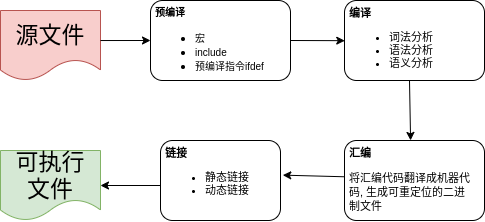
\includegraphics[scale=0.8]{pic1.png} \par
\section{链接的原因}
程序开发的过程中, 不会把所有的代码都跟主函数写在同一个$.cc$文件中,而是不同的模块功能实现在不同的文件中, 模块间的依赖以及主函数文件对其他模块的依赖通过$include$对应模块的头文件来实现.而在预编译$\rightarrow$编译$\rightarrow$汇编后, 对于每个模块,生成了自己对应的目标文件.最后需要将这些目标文件跟主函数所对应的目标文件"整合"到一起生成可执行文件,这个过程就是链接.
\section{静态链接}
\subsection{原理} 
静态链接就是在生成可执行文件的时候, 所有的目标文件经过重定位等一系列操作包含在最后的可执行文件中.假设有下面的源文件: \par

\begin{lstlisting}[language=C++, caption={hello.h}]
inline int Add(int a, int b) {
  return a + b;
}
\end{lstlisting}

\begin{lstlisting}[language=C++, caption={main.cc}]
#include <stdio.h>
#include "hello.h"

int main() {
  printf("Hello World\n");
  return 0;
}
\end{lstlisting}
那么生成的可执行文件如下图所示.最后的可执行文件包含了所有使用到的目标文件. \par
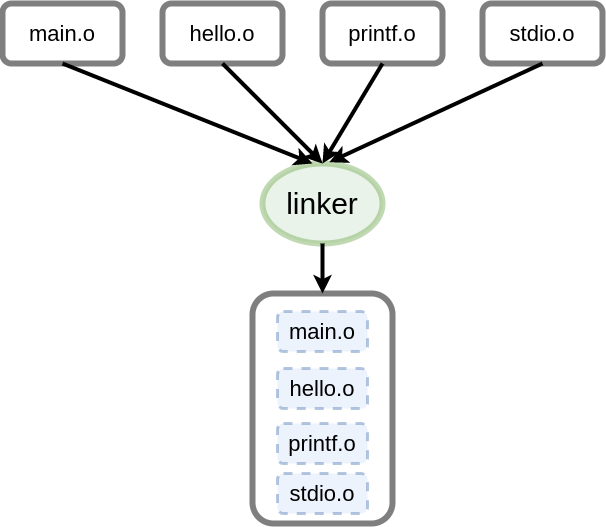
\includegraphics[scale=0.6]{pic2.png} \par

\subsection{优缺点} 
\begin{itemize}
	\item 优点是可移植性好, 因为不再依赖其他文件
	\item 第一个缺点文件太大
	\item 第二个缺点更新麻烦,如果一个模块更新,那么要重新链接生成可执行文件
	\item 第三个缺点如过一个模块被静态链接到多个可执行文件中,那么在运行这些程序的时候,这一个模块不能共享从而会占用很多内存
\end{itemize}
\section{动态链接}
\subsection{原理} 
动态链接是在运行的时候才把它使用的动态链接库进重定位等操作.而可执行文件在磁盘上的时候是不包含实际的目标文件的.在加载的时候去查找使用的动态链接库, 如果不在内存中, 那么将其加载到内存,并且进行重定位;如果在内存,那么将其映射到内存空间中.如下图所示: \par
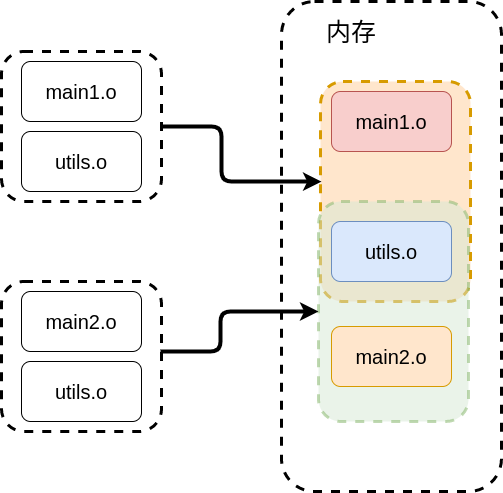
\includegraphics[scale=0.4]{pic3.png} \par
\subsection{优缺点} 
\begin{itemize}
	\item 第一个优点文件磁盘上的文件变小
	\item 第二个优点易更新
	\item 第三个优点可共享内存
	\item 第一个缺点移植性不好,从一台拷贝到另一台机器的时候,需要所有的动态链接库的位置一样
	\item 第二个缺点性能有所损失,因为要在运行的时候进行一些重定位操作
\end{itemize}
\end{document}
